\chapter{Технологическая часть}

\section{Выбор языка и среды программирования}

Для реализации программного обеспечения, выполняющего умножение матриц тремя алгоритмами, выбраны следующие инструменты и технические средства:

\begin{itemize}
	\item операционная система: Windows 10~\cite{lit4};
	\item среда разработки: Visual Studio Code~\cite{lit5};
	\item компилятор: \texttt{g++} версии 15.1.0~\cite{lit6};
	\item центральный процессор (CPU): Intel Core i5-11400H~\cite{lit7};
	\item оперативная память (RAM): 16 ГБ~\cite{lit8};
	\item язык программирования: C++17~\cite{lit9};
	\item библиотеки:
	\begin{itemize}
		\item стандартная библиотека STL~\cite{lit10} — контейнеры \texttt{vector}, ввод-вывод (\texttt{iomanip}, \texttt{iostream});
		\item библиотека \texttt{chrono}~\cite{lit11} — измерение времени выполнения алгоритмов;
		\item библиотека \texttt{fstream}~\cite{lit12} — запись результатов замеров производительности в CSV-файлы;
		\item генератор случайных чисел \texttt{<random>}~\cite{lit13} — заполнение матриц случайными элементами.
	\end{itemize}
\end{itemize}

Для реализации выбран язык программирования C++. Это обусловлено его высокой скоростью работы, возможностью прямого управления памятью и наличием средств для точного измерения времени выполнения программ. Эти свойства делают C++ удобным инструментом для проведения исследований и сравнения эффективности алгоритмов.

\section{Установка и настройка среды}

Компиляция проекта выполняется с помощью команды g++, 
что показано в листинге~\ref{lst:build}.

\begin{lstlisting}[language=bash, caption={Компиляция проекта}\raggedright, label={lst:build}]
	g++ main.cpp mult_algos.cpp matrix_utils.cpp -std=c++17 -o matrix_mult.exe
\end{lstlisting}

Для запуска программы используется команда, представленная в листинге~\ref{lst:run}.

\begin{lstlisting}[language=bash, caption={Запуск программы}\raggedright, label={lst:run}]
	./matrix_mult.exe
\end{lstlisting}

При запуске пользователь выбирает один из двух режимов:
\begin{itemize}
	\item ручной ввод матриц и вычисление результата;
	\item автоматическое сравнение времени работы трёх алгоритмов при разных размерах матриц.
\end{itemize}

\section{Реализация алгоритмов}

В данном разделе представлены реализации трёх алгоритмов умножения матриц: стандартного, алгоритма Винограда и его оптимизированной версии. Каждый алгоритм оформлен в виде отдельной функции на языке C++.

\subsection{Стандартный алгоритм}

Стандартный алгоритм умножения матриц основан на трёх вложенных циклах. Каждый элемент результирующей матрицы вычисляется как скалярное произведение строки первой матрицы и столбца второй. Код представлен в листинге~\ref{lst:standard}.

\begin{lstlisting}[language=C++, caption={Стандартный алгоритм умножения матриц}\raggedright, label={lst:standard}]
	Matrix mult_standard(const Matrix &A, const Matrix &B) 
	{
	    int n = A.size(), m = B[0].size(), k = B.size();
	    Matrix C(n, std::vector<int>(m, 0));
	    for (int i = 0; i < n; ++i)
	        for (int j = 0; j < m; ++j)
	            for (int t = 0; t < k; ++t)
	                C[i][j] += A[i][t] * B[t][j];
	    return C;
	}
\end{lstlisting}

\subsection{Алгоритм Винограда}

Алгоритм Винограда представляет собой усовершенствованный вариант стандартного способа умножения матриц, направленный на уменьшение количества арифметических операций. 
Основная идея данного метода заключается в использовании предварительных вычислений, позволяющих частично сократить число умножений, выполняемых в основном цикле. 

Перед началом основного этапа производится вычисление вспомогательных массивов для строк первой матрицы и для столбцов второй матрицы. Эти массивы содержат результаты промежуточных произведений, которые используются при формировании итоговых элементов результирующей матрицы. Такой подход позволяет снизить количество умножений за счёт замены части из них на операции сложения, что повышает общую эффективность алгоритма.  

Реализация алгоритма на языке C++ представлена в листинге~\ref{lst:vinograd}. 
Программная реализация сохраняет структуру базового метода, но дополнена этапами вычисления и использования вспомогательных массивов, что позволяет более рационально использовать ресурсы процессора и уменьшить время выполнения операции умножения.


\begin{lstlisting}[language=C++, caption={Алгоритм Винограда умножения матриц}\raggedright, label={lst:vinograd}]
	Matrix mult_vinograd(const Matrix &A, const Matrix &B) 
	{
	    int n = A.size(), m = B[0].size(), k = B.size();
	    Matrix C(n, std::vector<int>(m, 0));
	    std::vector<int> row_factor(n, 0), col_factor(m, 0);
	    for (int i = 0; i < n; ++i)
	        for (int t = 0; t < k/2; ++t)
	            row_factor[i] += A[i][2*t] * A[i][2*t+1];
	    for (int j = 0; j < m; ++j)
	        for (int t = 0; t < k/2; ++t)
	            col_factor[j] += B[2*t][j] * B[2*t+1][j];
	    for (int i = 0; i < n; ++i) 
	        for (int j = 0; j < m; ++j)
	        {
	            C[i][j] = -row_factor[i] - col_factor[j];
	            for (int t = 0; t < k/2; ++t)
	                C[i][j] += (A[i][2*t] + B[2*t+1][j]) *
	                           (A[i][2*t+1] + B[2*t][j]);
	        }
	    if (k % 2 == 1) 
	        for (int i = 0; i < n; ++i)
	            for (int j = 0; j < m; ++j)
	                C[i][j] += A[i][k-1] * B[k-1][j];
	
	    return C;
	}
\end{lstlisting}

\subsection{Оптимизированный алгоритм Винограда}

Оптимизированный вариант алгоритма Винограда содержит ряд дополнительных усовершенствований, направленных на повышение эффективности вычислений. Основные изменения включают вынесение повторяющихся выражений в отдельные переменные, использование локальных аккумуляторов и уменьшение числа обращений к памяти, что снижает вычислительные затраты. Благодаря этим доработкам достигается более высокая скорость выполнения программы при сохранении точности результатов. Фрагмент реализации алгоритма представлен в листинге~\ref{lst:vinograd_opt}.

\begin{lstlisting}[language=C++, caption={Оптимизированный алгоритм Винограда}\raggedright, label={lst:vinograd_opt}]
	Matrix mult_vinograd_opt(const Matrix &A, const Matrix &B) 
	{
	    int n = A.size(), m = B[0].size(), k = B.size();
	    Matrix C(n, std::vector<int>(m, 0));
	    std::vector<int> row_factor(n, 0), col_factor(m, 0);
	    int k2 = k / 2;
	    for (int i = 0; i < n; ++i) 
	    {
	        int sum = 0;
	        for (int t = 0; t < k2; ++t)
	            sum += A[i][2*t] * A[i][2*t+1];
	        row_factor[i] = sum;
	    }
	    for (int j = 0; j < m; ++j) 
	    {
	        int sum = 0;
	        for (int t = 0; t < k2; ++t)
	            sum += B[2*t][j] * B[2*t+1][j];
	        col_factor[j] = sum;
	    }
	    for (int i = 0; i < n; ++i)
	        for (int j = 0; j < m; ++j) 
	        {
	            int temp = -row_factor[i] - col_factor[j];
	            for (int t = 0; t < k2; ++t)
	                temp += (A[i][2*t] + B[2*t+1][j]) *
	                        (A[i][2*t+1] + B[2*t][j]);
	            C[i][j] = temp;
	        }
	    if (k % 2 == 1) 
	    {
	        int last = k-1;
	        for (int i = 0; i < n; ++i)
	            for (int j = 0; j < m; ++j)
	                C[i][j] += A[i][last] * B[last][j];
	    }
	    return C;
	}
\end{lstlisting}

\section{Результаты работы}

Разработанная программа поддерживает два режима работы: режим ручного ввода данных и режим автоматического измерения времени выполнения алгоритмов.  

В режиме ручного ввода пользователь задаёт размеры матриц и их элементы с клавиатуры. 
Программа выполняет умножение матриц с использованием трёх методов: стандартного алгоритма, алгоритма Винограда и его оптимизированной версии. 
Результаты вычислений выводятся в консоль в виде матриц. 
Пример работы программы в данном режиме представлен на рисунке~\ref{fig:mode1}.  

\begin{figure}[H]
	\centering
	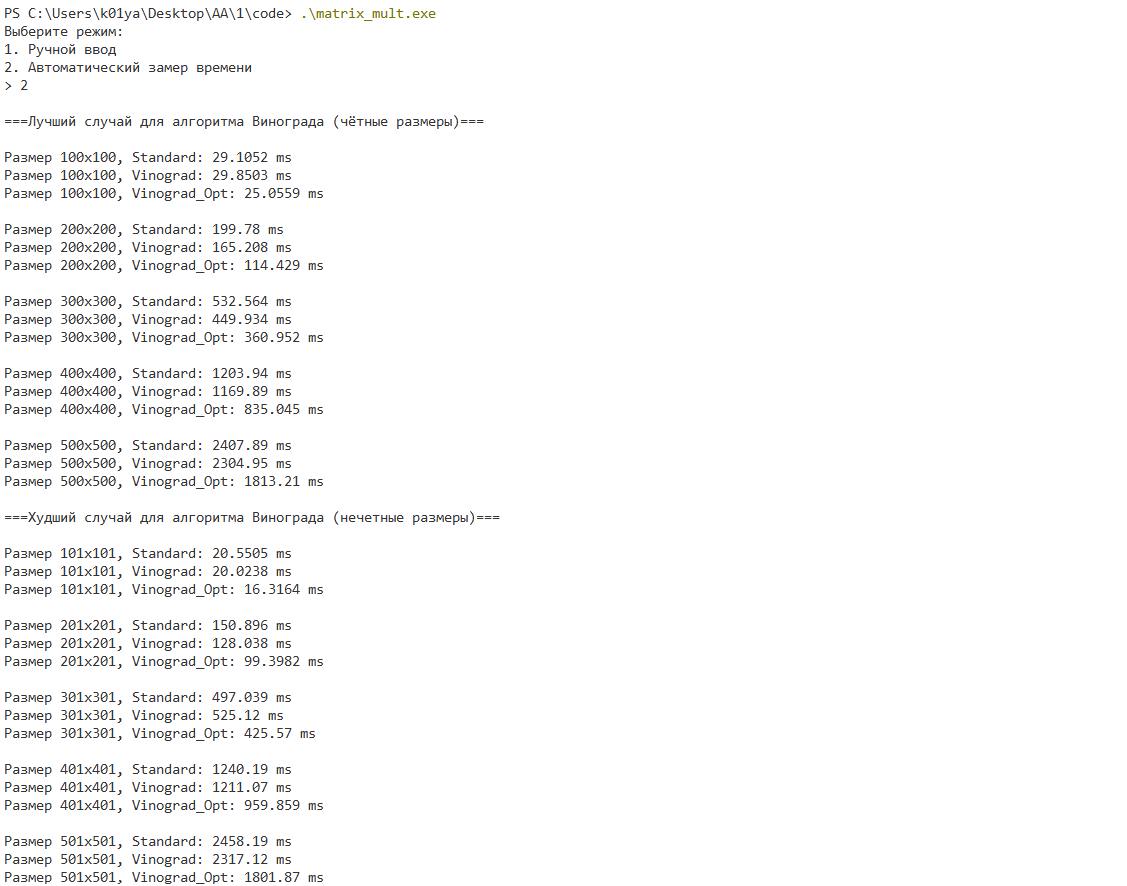
\includegraphics[width=0.84\linewidth]{res1.png}
	\caption{Пример работы программы в режиме ручного ввода матриц}
	\label{fig:mode1}
\end{figure}

Во втором режиме осуществляется автоматический замер времени выполнения алгоритмов.Пример вывода программы в этом режиме показан на рисунке~\ref{fig:mode2}.  

\begin{figure}[H]
	\centering
	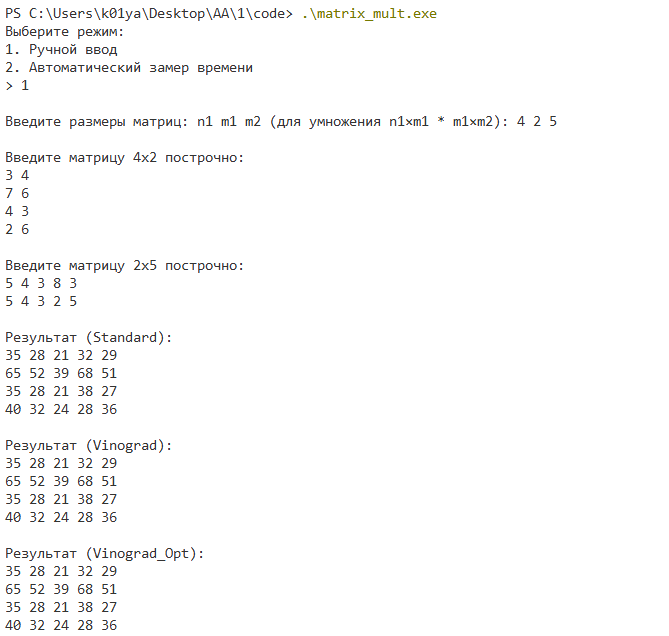
\includegraphics[width=0.84\linewidth]{res2.png}
	\caption{Пример работы программы в режиме автоматического замера времени}
	\label{fig:mode2}
\end{figure}

Полученные данные показывают устойчивую тенденцию к ускорению при использовании оптимизированной версии, что подтверждает эффективность предложенных улучшений.

\section*{Вывод}

В ходе работы были выбраны инструменты разработки и обоснован выбор языка программирования C++. 
Программа реализована по модульному принципу, что позволяет разделить логику обработки матриц и реализацию алгоритмов умножения.  

Программное обеспечение обеспечивает два режима работы: 
ручной ввод матриц с выводом результата и автоматическое измерение времени выполнения алгоритмов.  
Полученные реализации позволяют провести сравнение производительности стандартного алгоритма, алгоритма Винограда и его оптимизированной версии, а также подтвердить эффективность внесённых оптимизаций.

\clearpage

